\documentclass[a4paper,12pt]{article}
\usepackage[utf8]{inputenc}
\usepackage{graphicx}
\usepackage[margin=1in]{geometry}
\usepackage{titling}
\usepackage{fancyhdr} % header and footer
\usepackage{everypage}
\usepackage{hyperref}
\usepackage{array}
\usepackage{xcolor}
\graphicspath{ {./images} }
\definecolor{linkblue}{RGB}{0, 0, 255}

\hypersetup{
    colorlinks=false,
}

\fancypagestyle{plain}{ 
    \fancyhf{}
    \renewcommand{\headrulewidth}{0pt}
    \renewcommand{\footrulewidth}{0pt}
}

\fancyhf{}
\fancyhead[L]{
\includegraphics[width=0.3\textwidth]{logo_ipl.png}}
\fancyhead[R]{
    \small Licenciatura em Eng. Informática\\
    Ano Letivo 2024/2025\\
    Sistemas Gráficos e Interação -- Projeto
}
\setlength{\headsep}{2cm}
\renewcommand{\headrulewidth}{0pt}
\renewcommand{\contentsname}{Índice}

\fancyfoot[R]{\thepage} 
\setlength{\footskip}{0cm}
\pagestyle{fancy}

\begin{document}

\begin{titlepage}
    \begin{center}
        
\includegraphics[width=0.5\textwidth]{logo_ipl.png}
    \end{center}

    \vspace{1cm}

    \begin{center}
        \fboxsep=10pt
        \parbox[c][3cm][c]{0.8\textwidth}{
            \centering
            \textbf{\Large Relatório do Projeto de}\\[0.3cm]
            \textbf{\Large Interface web 3D}
        }
    \end{center}

    \vfill

    \begin{center}
        \textbf{Licenciatura em Engenharia Informática}\\
        Sistemas Gráficos e Interação\\[0.5cm]
        \vspace{1cm}
        \textbf{Ano Letivo: 2024/2025}
    \end{center}

    \vfill

    % Student information
    \begin{center}
        \textbf{Estudantes:}\\[0.3cm]
        Marco Padeiro, 2231953\\
        Rodrigo Carreira, 2231952
    \end{center}
    \thispagestyle{plain}
\end{titlepage}

\newpage
\tableofcontents

\newpage
\section{Avaliação heurística}

\begin{center}

    \begin{table}[h!]
        \centering
        \begin{tabular}{|m{3cm}|m{12cm}|}
            \hline
            \multicolumn{2}{|c|}{\textbf{Registo 1}}                                                                                                               \\ \hline
            \textbf{Tarefa}       & Acesso a página de Login/Registo                                                                                               \\ \hline
            \textbf{Local}        & Ao abrir a página de Login/Registo                                                                                             \\ \hline
            \textbf{Heurística}   & 4                                                                                                                              \\ \hline
            \textbf{Descrição}    & O footer presente nesta página não se encontra no fundo da página.                                                             \\ \hline
            \textbf{Frequência}   & Apenas uma vez                                                                                                                 \\ \hline
            \textbf{Persistência} & Persistente                                                                                                                    \\ \hline
            \textbf{Severidade}   & 1                                                                                                                              \\ \hline
            \textbf{Solução}      & Fazer com que o footer fique no fundo da página mesmo que está não tenha conteudo sufiente para preencher uma página completa. \\ \hline
        \end{tabular}
    \end{table}

    \vspace{0.5cm}
    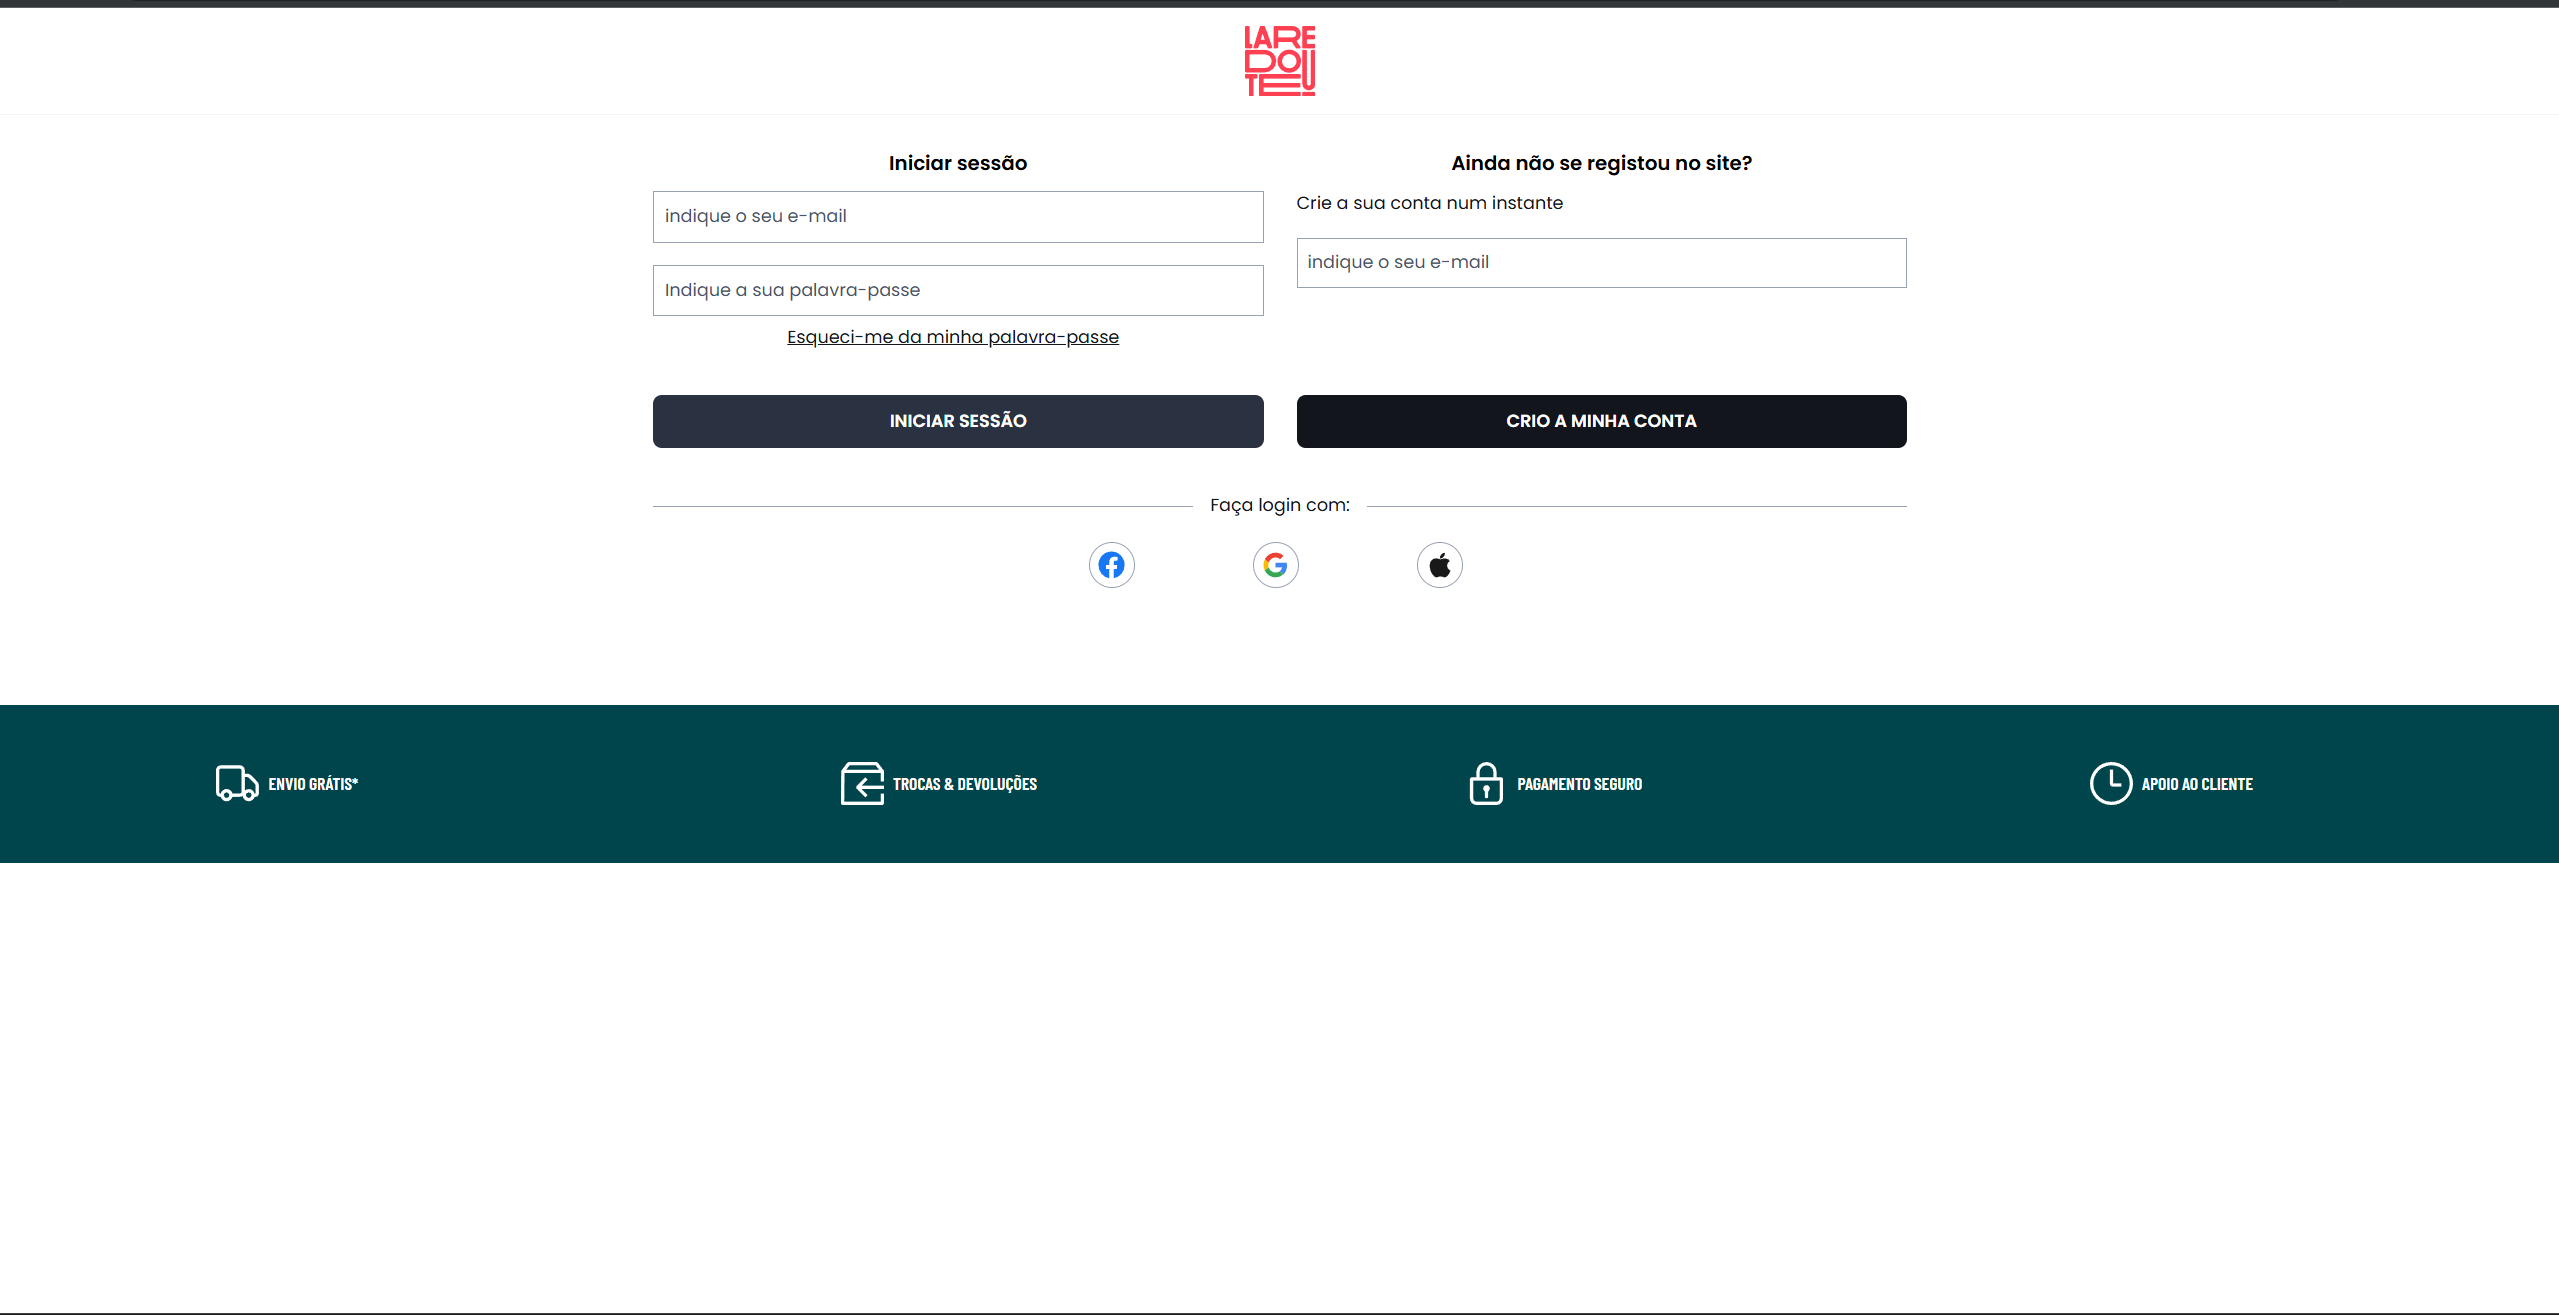
\includegraphics[width=\textwidth, keepaspectratio]{heuristics/01footer_registo.png}


    \newpage
    \begin{table}[h!]
        \centering
        \begin{tabular}{|m{3cm}|m{12cm}|}
            \hline
            \multicolumn{2}{|c|}{\textbf{Registo 2}}                                                                                                               \\ \hline
            \textbf{Tarefa}       & Visualizar detalhes do produto.                                                                                                \\ \hline
            \textbf{Local}        & Ao editar a quantidade pretendida de um produto.                                                                               \\ \hline
            \textbf{Heurística}   & 4                                                                                                                              \\ \hline
            \textbf{Descrição}    & A utilização de um input numérico com botões de '+' e '-' é mais intuitiva e standard do que o uso de um input do tipo select. \\ \hline
            \textbf{Frequência}   & Sempre                                                                                                                         \\ \hline
            \textbf{Persistência} & Persistente                                                                                                                    \\ \hline
            \textbf{Severidade}   & 0                                                                                                                              \\ \hline
            \textbf{Solução}      & Utilizar um input numérico com limite variável conforme o produto e botões de incremento.                                      \\ \hline
        \end{tabular}
    \end{table}

    \begin{table}[h!]
        \centering
        \begin{tabular}{|m{3cm}|m{12cm}|}
            \hline
            \multicolumn{2}{|c|}{\textbf{Registo 3}}                                                                                                      \\ \hline
            \textbf{Tarefa}       & Visualizar detalhes do produto.                                                                                       \\ \hline
            \textbf{Local}        & Ao editar a quantidade pretendida de um produto.                                                                      \\ \hline
            \textbf{Heurística}   & 8                                                                                                                     \\ \hline
            \textbf{Descrição}    & A utilização de um input numérico com botões de '+' e '-' é mais minimalista do que o uso de um input do tipo select. \\ \hline
            \textbf{Frequência}   & Sempre                                                                                                                \\ \hline
            \textbf{Persistência} & Persistente                                                                                                           \\ \hline
            \textbf{Severidade}   & 0                                                                                                                     \\ \hline
            \textbf{Solução}      & Utilizar um input numérico com limite variável conforme o produto e botões de incremento.                             \\ \hline
        \end{tabular}
    \end{table}
    \vspace{0.5cm}
    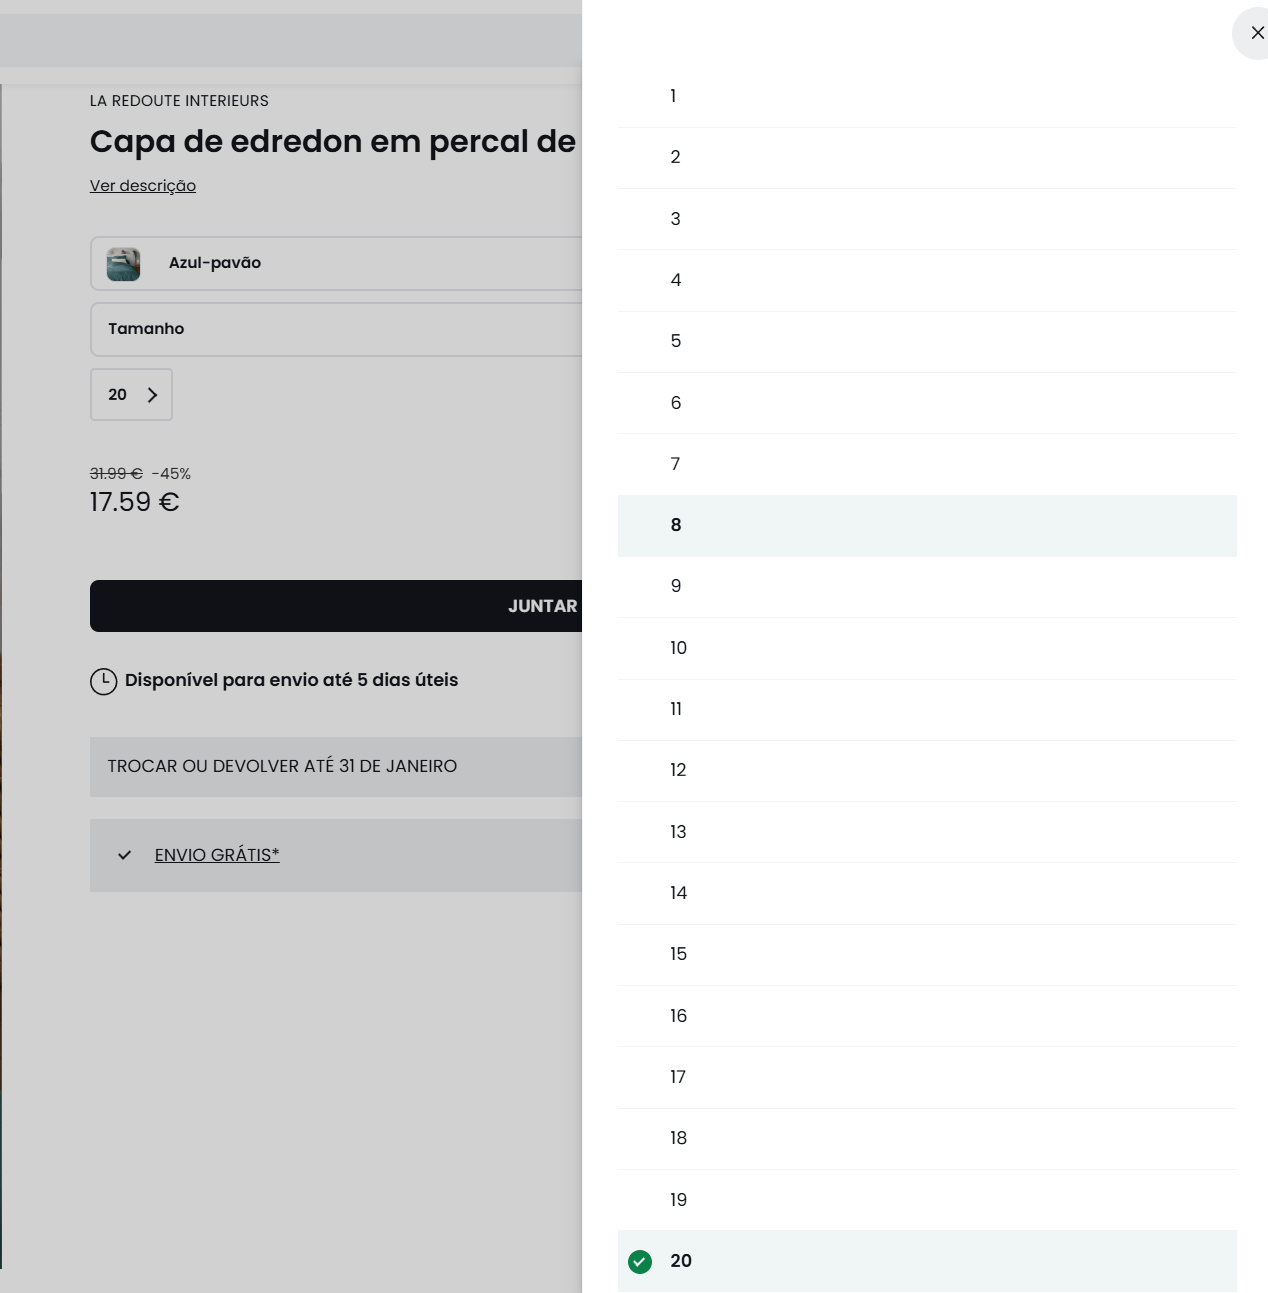
\includegraphics[width=0.7\textwidth]{heuristics/02input_quantidade.png}

    \newpage
    \begin{table}[h!]
        \centering
        \begin{tabular}{|m{3cm}|m{12cm}|}
            \hline
            \multicolumn{2}{|c|}{\textbf{Registo 4}}                                                \\ \hline
            \textbf{Tarefa}       & Acedar ao carrinho                                              \\ \hline
            \textbf{Local}        & Página de carrinho                                              \\ \hline
            \textbf{Heurística}   & 4                                                               \\ \hline
            \textbf{Descrição}    & Os breadcrumbs estão muito próximos da margem da página.        \\ \hline
            \textbf{Frequência}   & Sempre                                                          \\ \hline
            \textbf{Persistência} & Persistente                                                     \\ \hline
            \textbf{Severidade}   & 1                                                               \\ \hline
            \textbf{Solução}      & Adicionar uma margem entre o início da página e os breadcrumbs. \\ \hline
        \end{tabular}
    \end{table}

    \vspace{0.5cm}
    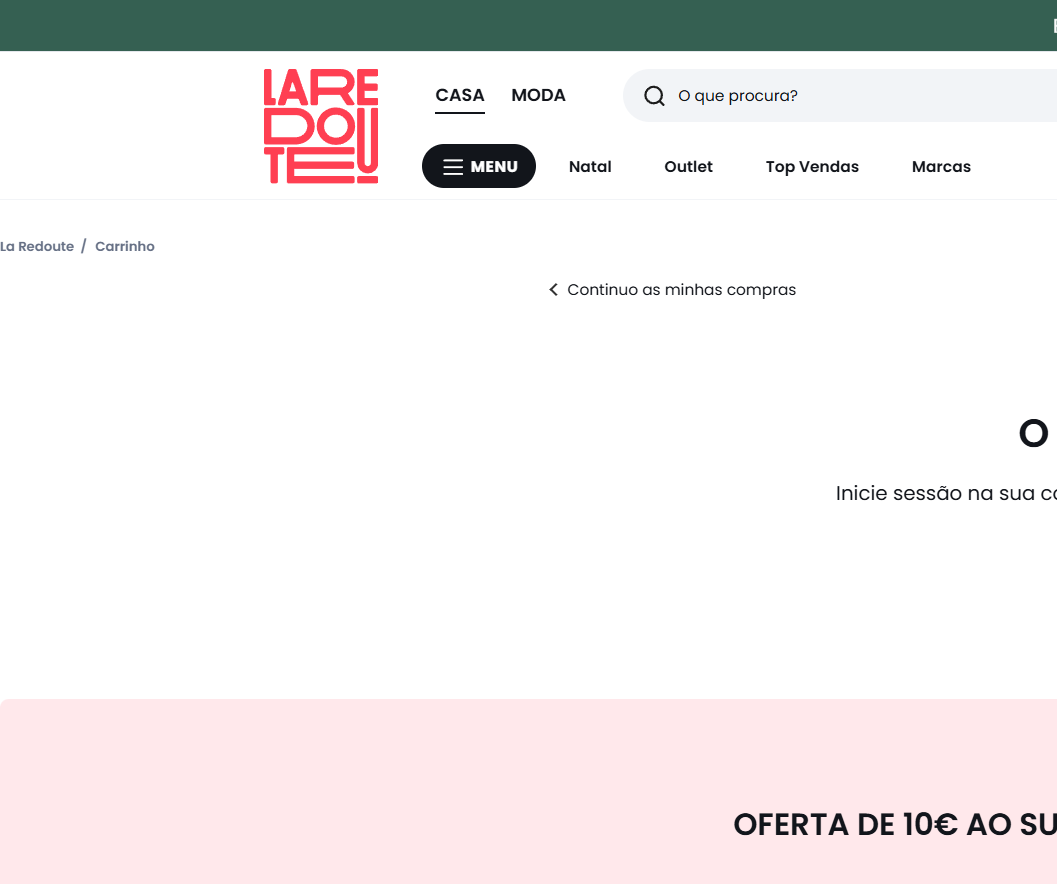
\includegraphics[width=\textwidth, keepaspectratio]{heuristics/03breadcrumbs_carrinho.png}

    \newpage
    \begin{table}[h!]
        \centering
        \begin{tabular}{|m{3cm}|m{12cm}|}
            \hline
            \multicolumn{2}{|c|}{\textbf{Registo 5}}                                                                       \\ \hline
            \textbf{Tarefa}       & Criar uma conta                                                                        \\ \hline
            \textbf{Local}        & Ao aceder a página de Registo                                                          \\ \hline
            \textbf{Heurística}   & 5                                                                                      \\ \hline
            \textbf{Descrição}    & A distinção entre particular e empresa é feita no campo de gênero.                     \\ \hline
            \textbf{Frequência}   & Apenas uma vez                                                                         \\ \hline
            \textbf{Persistência} & Persistente                                                                            \\ \hline
            \textbf{Severidade}   & 2                                                                                      \\ \hline
            \textbf{Solução}      & Adicionar um novo campo de input para realizar a distinção entre particular e empresa. \\ \hline
        \end{tabular}
    \end{table}

    \vspace{0.5cm}
    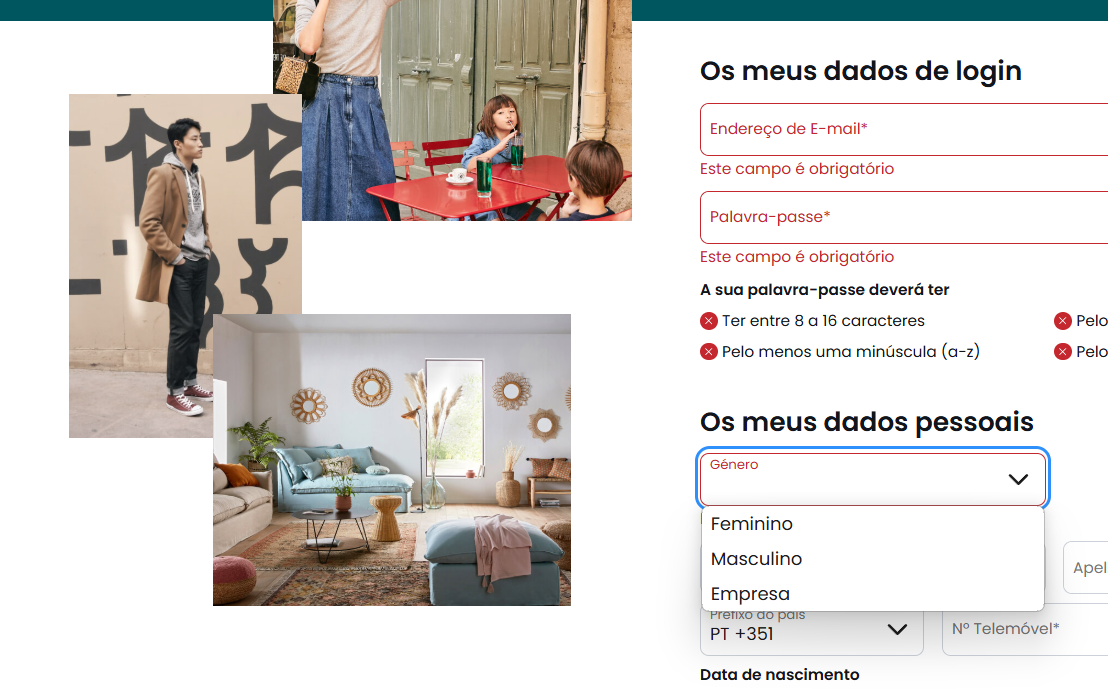
\includegraphics[width=\textwidth, keepaspectratio]{heuristics/04genero_registo.png}

    \newpage
    \begin{table}[h!]
        \centering
        \begin{tabular}{|m{3cm}|m{12cm}|}
            \hline
            \multicolumn{2}{|c|}{\textbf{Registo 6}}                                                                                                     \\ \hline
            \textbf{Tarefa}       & Abrir a página inicial                                                                                               \\ \hline
            \textbf{Local}        & Página principal do website                                                                                          \\ \hline
            \textbf{Heurística}   & 8                                                                                                                    \\ \hline
            \textbf{Descrição}    & O banner animado é excessivamente grande em relação à pouca informação que apresenta, ofuscando o restante conteúdo. \\ \hline
            \textbf{Frequência}   & Sempre                                                                                                               \\ \hline
            \textbf{Persistência} & Persistente                                                                                                          \\ \hline
            \textbf{Severidade}   & 1                                                                                                                    \\ \hline
            \textbf{Solução}      & Reduzir o tamanho deste banner.                                                                                      \\ \hline
        \end{tabular}
    \end{table}

    \vspace{0.5cm}
    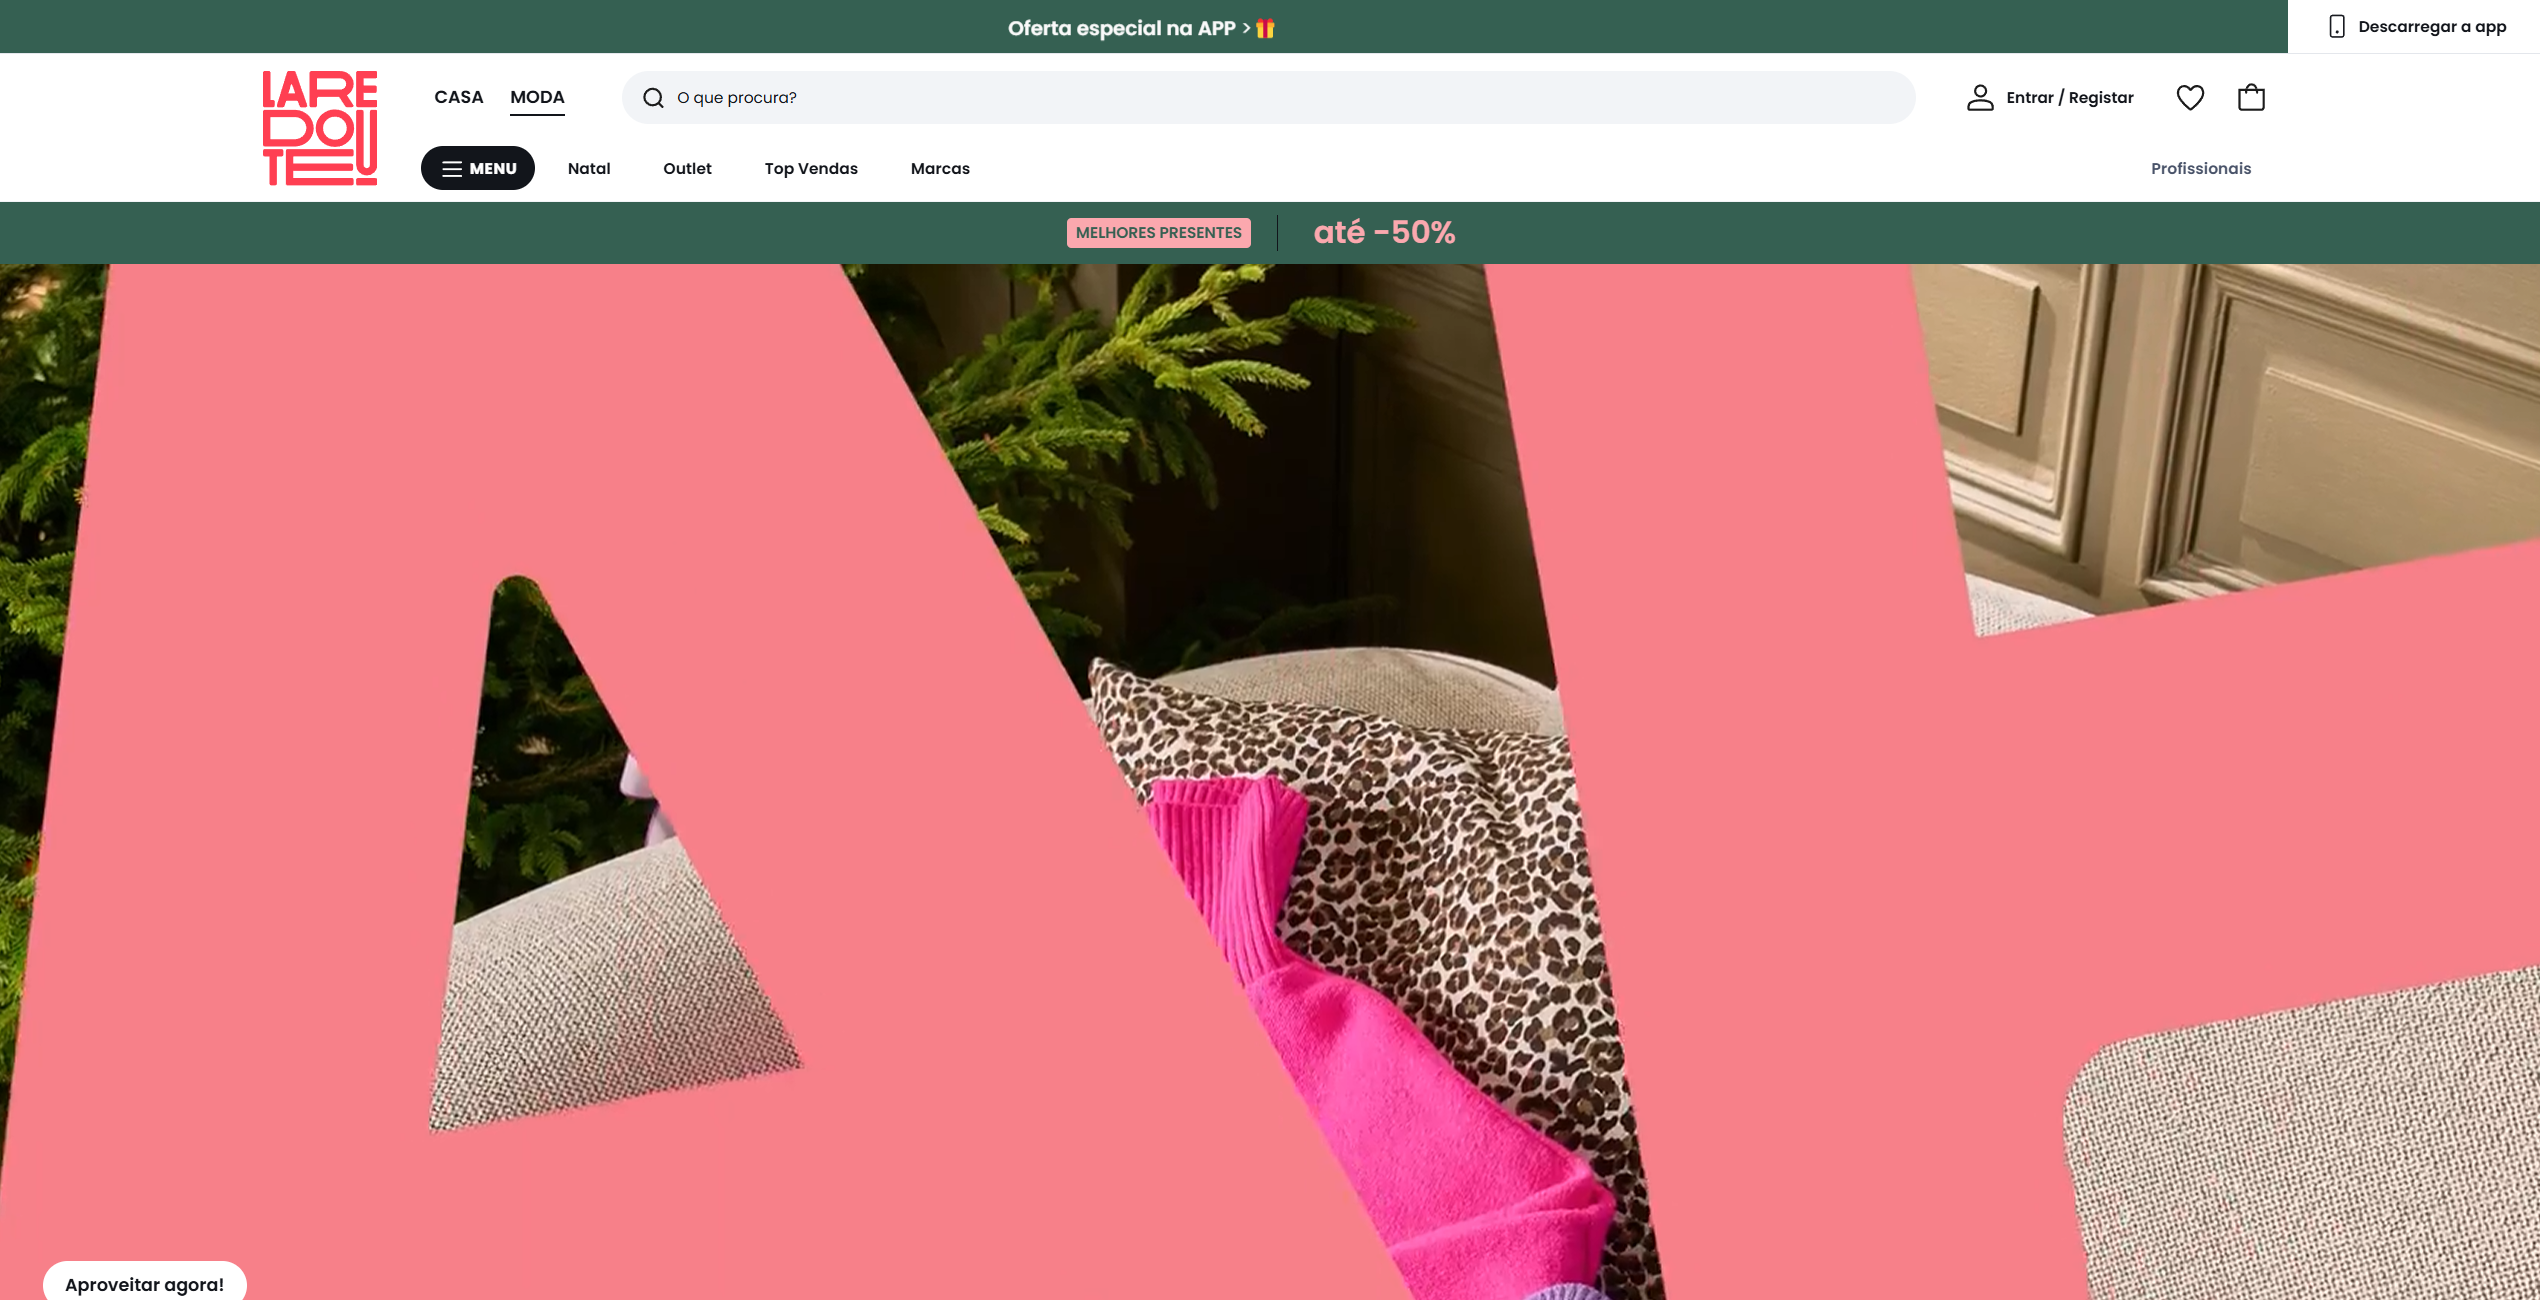
\includegraphics[width=\textwidth, keepaspectratio]{heuristics/05informacao_homepage.png}

    \newpage
    \begin{table}[h!]
        \centering
        \begin{tabular}{|m{3cm}|m{12cm}|}
            \hline
            \multicolumn{2}{|c|}{\textbf{Registo 7}}                                                                              \\ \hline
            \textbf{Tarefa}       & Criação de conta                                                                              \\ \hline
            \textbf{Local}        & Página de registo                                                                             \\ \hline
            \textbf{Heurística}   & 3                                                                                             \\ \hline
            \textbf{Descrição}    & O campo do número de telemóvel e o campo da morada não são opcionais.                         \\ \hline
            \textbf{Frequência}   & Sempre                                                                                        \\ \hline
            \textbf{Persistência} & Persistente                                                                                   \\ \hline
            \textbf{Severidade}   & 0                                                                                             \\ \hline
            \textbf{Solução}      & Deixar estas informações como opcionais e torná-las obrigatórias apenas ao realizar a compra. \\ \hline
        \end{tabular}
    \end{table}

    \vspace{0.5cm}
    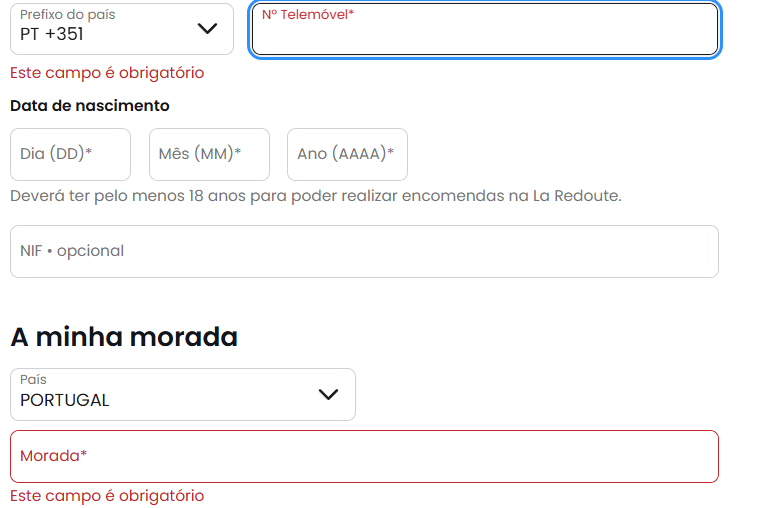
\includegraphics[width=\textwidth, keepaspectratio]{heuristics/06telefone_registo.png}

    \newpage
    \begin{table}[h!]
        \centering
        \begin{tabular}{|m{3cm}|m{12cm}|}
            \hline
            \multicolumn{2}{|c|}{\textbf{Registo 8}}                                                                                          \\ \hline
            \textbf{Tarefa}       & Remover um produto de carrinho                                                                            \\ \hline
            \textbf{Local}        & Página do carrinho                                                                                        \\ \hline
            \textbf{Heurística}   & 5                                                                                                         \\ \hline
            \textbf{Descrição}    & Não há nenhuma confirmação ao tentar remover um artigo do carrinho, podendo levar à remoção por acidente. \\ \hline
            \textbf{Frequência}   & Sempre                                                                                                    \\ \hline
            \textbf{Persistência} & Persistente                                                                                               \\ \hline
            \textbf{Severidade}   & 2                                                                                                         \\ \hline
            \textbf{Solução}      & Adicionar um pop up de confirmação.                                                                       \\ \hline
        \end{tabular}
    \end{table}

    \begin{table}[h!]
        \centering
        \begin{tabular}{|m{3cm}|m{12cm}|}
            \hline
            \multicolumn{2}{|c|}{\textbf{Registo 9}}                                                                                                                                  \\ \hline
            \textbf{Tarefa}       & Remover um produto de carrinho                                                                                                                    \\ \hline
            \textbf{Local}        & Página do carrinho                                                                                                                                \\ \hline
            \textbf{Heurística}   & 9                                                                                                                                                 \\ \hline
            \textbf{Descrição}    & Não há nenhuma confirmação ao tentar remover um artigo do carrinho, caso houvesse a confirmação ajudaria a recuperar entes de remover sem querer. \\ \hline
            \textbf{Frequência}   & Sempre                                                                                                                                            \\ \hline
            \textbf{Persistência} & Persistente                                                                                                                                       \\ \hline
            \textbf{Severidade}   & 2                                                                                                                                                 \\ \hline
            \textbf{Solução}      & Adicionar um pop up de confirmação.                                                                                                               \\ \hline
        \end{tabular}
    \end{table}

    \vspace{0.5cm}
    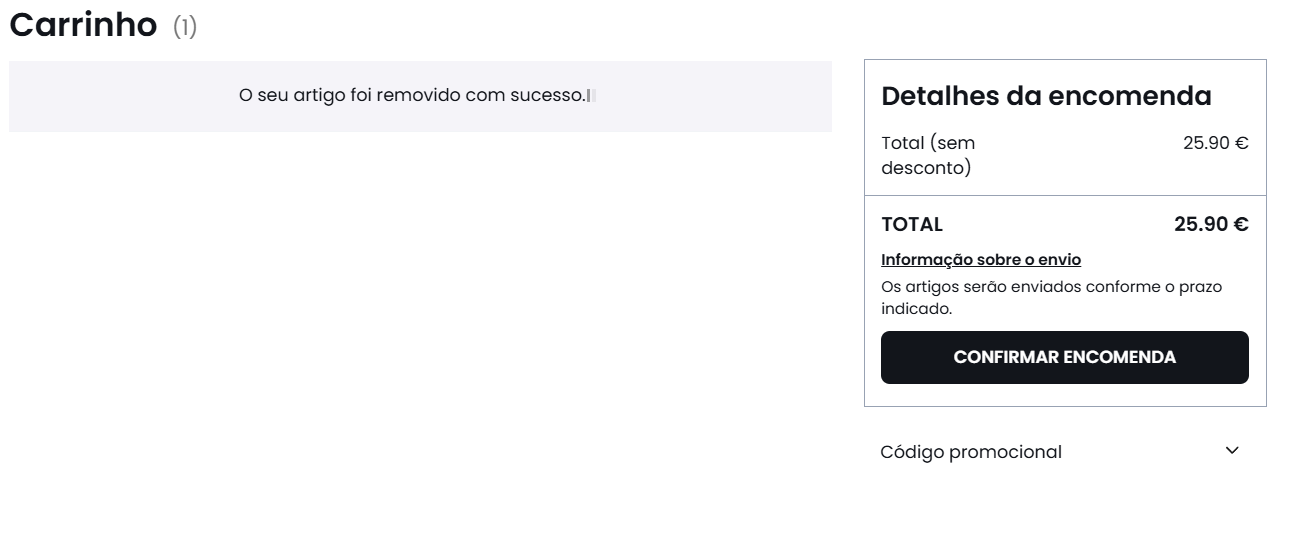
\includegraphics[width=\textwidth, keepaspectratio]{heuristics/07confirmacao_carrinho.png}

    \newpage
    \begin{table}[h!]
        \centering
        \begin{tabular}{|m{3cm}|m{12cm}|}
            \hline
            \multicolumn{2}{|c|}{\textbf{Registo 10}}                                                                                                   \\ \hline
            \textbf{Tarefa}       & Ao efetuar o registo                                                                                                \\ \hline
            \textbf{Local}        & Página do registo                                                                                                   \\ \hline
            \textbf{Heurística}   & 5                                                                                                                   \\ \hline
            \textbf{Descrição}    & Não há nenhuma validação para o código postal, levando a possiveis abusos no sistema com códigos postais inválidos. \\ \hline
            \textbf{Frequência}   & Apenas uma vez                                                                                                      \\ \hline
            \textbf{Persistência} & Persistente                                                                                                         \\ \hline
            \textbf{Severidade}   & 3                                                                                                                   \\ \hline
            \textbf{Solução}      & Adicionar validação a este campo.                                                                                   \\ \hline
        \end{tabular}
    \end{table}

    \begin{table}[h!]
        \centering
        \begin{tabular}{|m{3cm}|m{12cm}|}
            \hline
            \multicolumn{2}{|c|}{\textbf{Registo 11}}                                                                                                                              \\ \hline
            \textbf{Tarefa}       & Ao efetuar o registo                                                                                                                           \\ \hline
            \textbf{Local}        & Página do registo                                                                                                                              \\ \hline
            \textbf{Heurística}   & 9                                                                                                                                              \\ \hline
            \textbf{Descrição}    & Não há nenhuma validação para o código postal, fazendo com que o utilizador não consiga corrigir para um código postal válido caso faça erros. \\ \hline
            \textbf{Frequência}   & Apenas uma vez                                                                                                                                 \\ \hline
            \textbf{Persistência} & Persistente                                                                                                                                    \\ \hline
            \textbf{Severidade}   & 3                                                                                                                                              \\ \hline
            \textbf{Solução}      & Adicionar validação a este campo.                                                                                                              \\ \hline
        \end{tabular}
    \end{table}

    \vspace{0.5cm}
    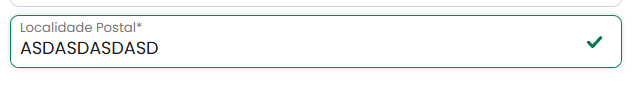
\includegraphics[width=\textwidth, keepaspectratio]{heuristics/08validacao_postal_registo.png}
\end{center}
\newpage

\subsection*{Resumo da avaliação heurística}
\begin{table}[h!]
    \centering
    \begin{tabular}{|m{0.5cm}|m{12cm}|m{0.5cm}|}
        \hline
        \multicolumn{3}{|c|}{\textbf{Heurística}}                               \\ \hline
        \textbf{1}  & Visibilidade do estado do sistema                     & 0 \\ \hline
        \textbf{2}  & Correspondência entre o sistema e o mundo real        & 0 \\ \hline
        \textbf{3}  & Liberdade e controlo pelo utilizador                  & 1 \\ \hline
        \textbf{4}  & Consistência e standards                              & 3 \\ \hline
        \textbf{5}  & Prevenção de erros                                    & 3 \\ \hline
        \textbf{6}  & Reconhecer em vez de relembrar                        & 0 \\ \hline
        \textbf{7}  & Flexibilidade e eficiência de utilização              & 0 \\ \hline
        \textbf{8}  & Estética e desenho minimalista                        & 2 \\ \hline
        \textbf{9}  & Ajuda utilizadores a reconhecer e recuperar dos erros & 2 \\ \hline
        \textbf{10} & Ajuda e documentação                                  & 0 \\ \hline
    \end{tabular}
\end{table}

\begin{table}[h!]
    \centering
    \begin{tabular}{|m{0.5cm}|m{12cm}|m{0.5cm}|}
        \hline
        \multicolumn{3}{|c|}{\textbf{Severidade}}                                   \\ \hline
        \textbf{0} & Não existe consenso de que seja um problema de usabilidade & 3 \\ \hline
        \textbf{1} & Problema cosmético                                         & 3 \\ \hline
        \textbf{2} & Problema menor                                             & 3 \\ \hline
        \textbf{3} & Problema significativo                                     & 2 \\ \hline
        \textbf{4} & Problema catastrófico                                      & 0 \\ \hline
    \end{tabular}
\end{table}

\newpage
\section{Análise de Utilizadores e Tarefas}

\begin{center}
    \textcolor{linkblue}{\href{https://forms.gle/mGgTZJcjzfStsLvn6}{Link para o formulário}}

    \vspace{0.3cm}
    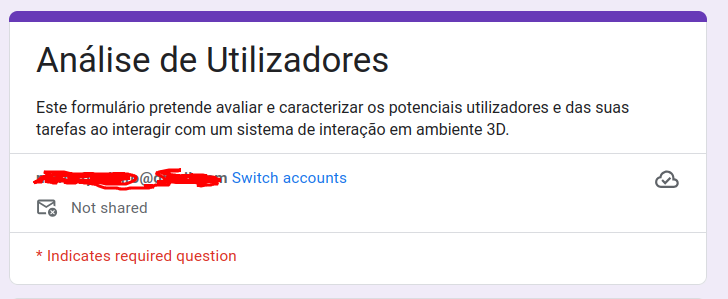
\includegraphics[width=0.75\textwidth]{form/intro_form.png}
    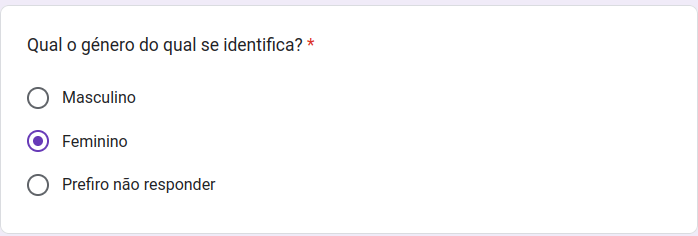
\includegraphics[width=0.75\textwidth]{form/01questao_genero.png}
    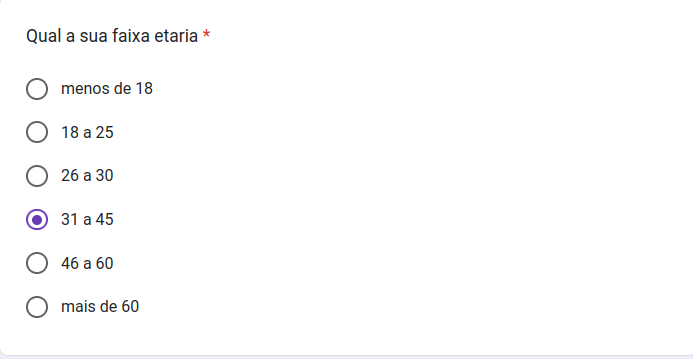
\includegraphics[width=0.75\textwidth]{form/02questao_idade.png}
    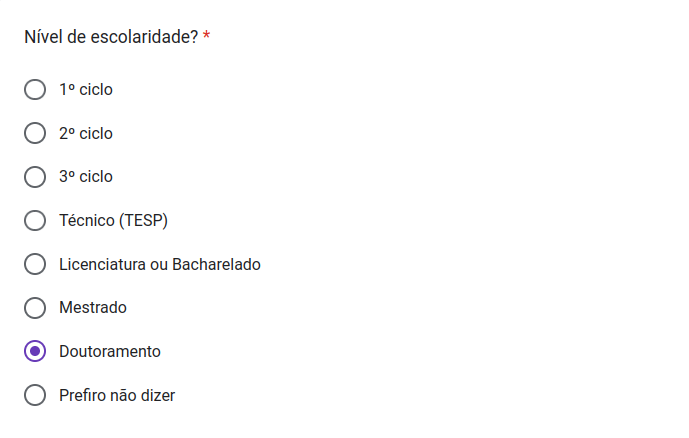
\includegraphics[width=0.75\textwidth]{form/03questao_escolaridade.png}
    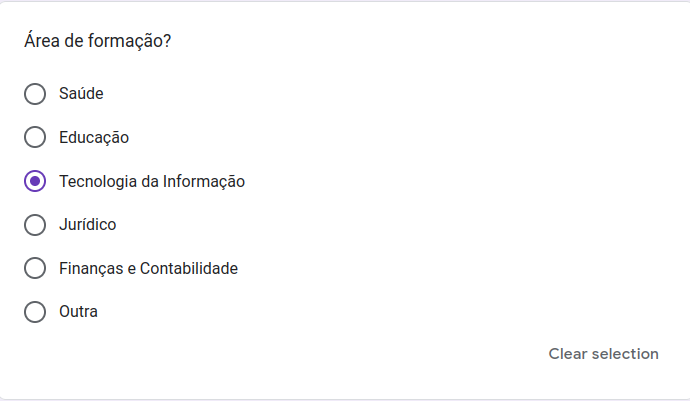
\includegraphics[width=0.75\textwidth]{form/04questao_formacao.png}
    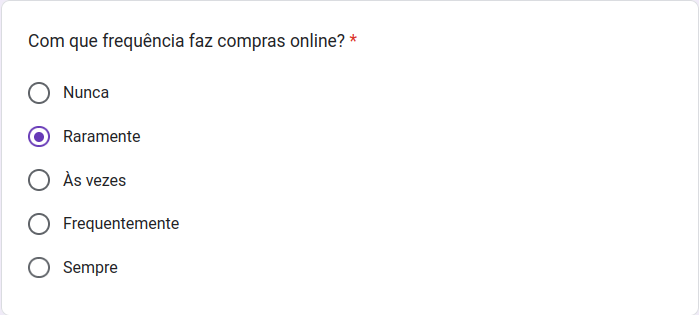
\includegraphics[width=0.75\textwidth]{form/05questao_comprasonline.png}
    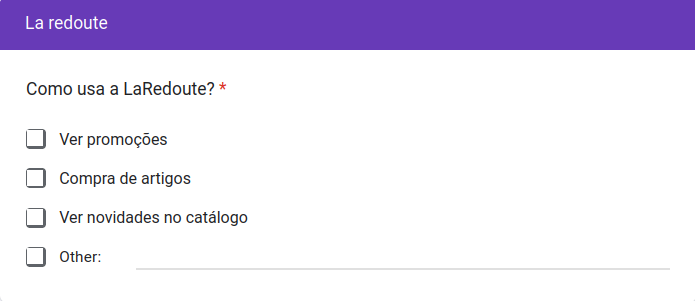
\includegraphics[width=0.75\textwidth]{form/06questao_usolaredoute.png}
    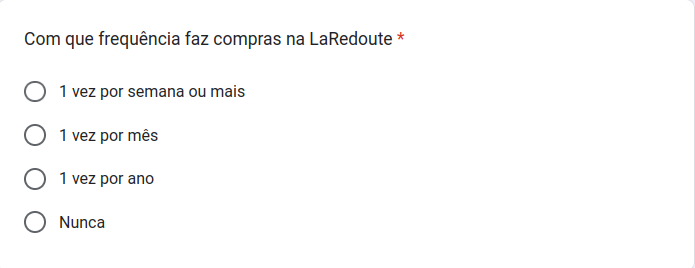
\includegraphics[width=0.75\textwidth]{form/07questao_frequencialaredoute.png}
    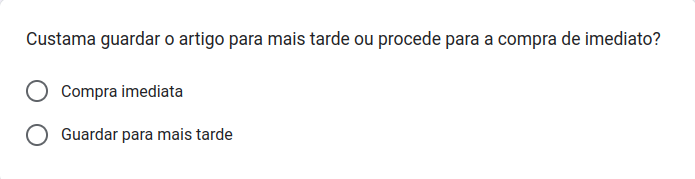
\includegraphics[width=0.75\textwidth]{form/08questao_guardarparatarde.png}
    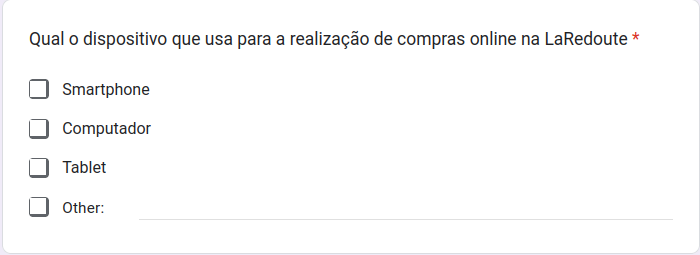
\includegraphics[width=0.75\textwidth]{form/09questao_dispositivocompra.png}
    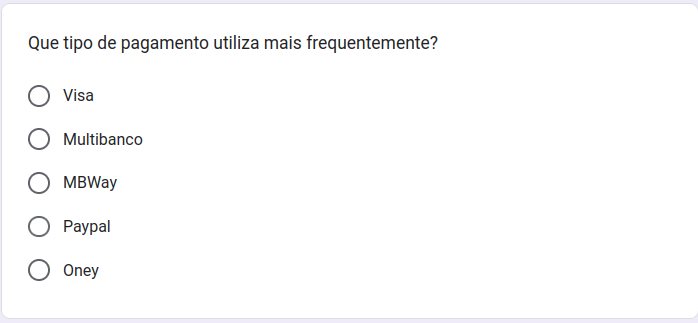
\includegraphics[width=0.75\textwidth]{form/10questao_metodopagamento.png}
    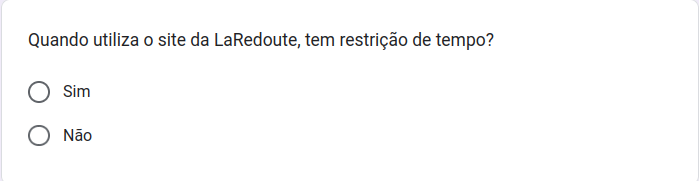
\includegraphics[width=0.75\textwidth]{form/11questao_restricaotempo.png}
    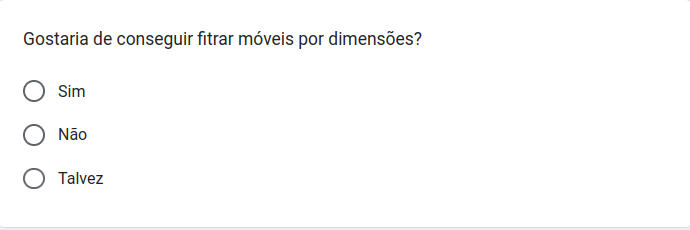
\includegraphics[width=0.75\textwidth]{form/12questao_filtrardimensoes.png}
    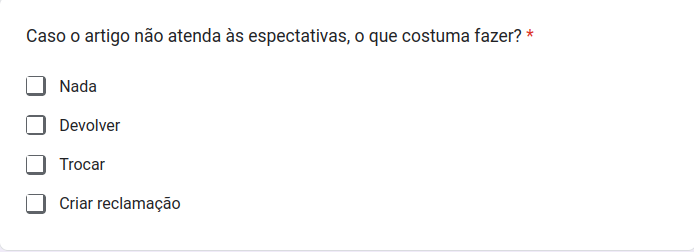
\includegraphics[width=0.75\textwidth]{form/13questao_expectativas.png}
    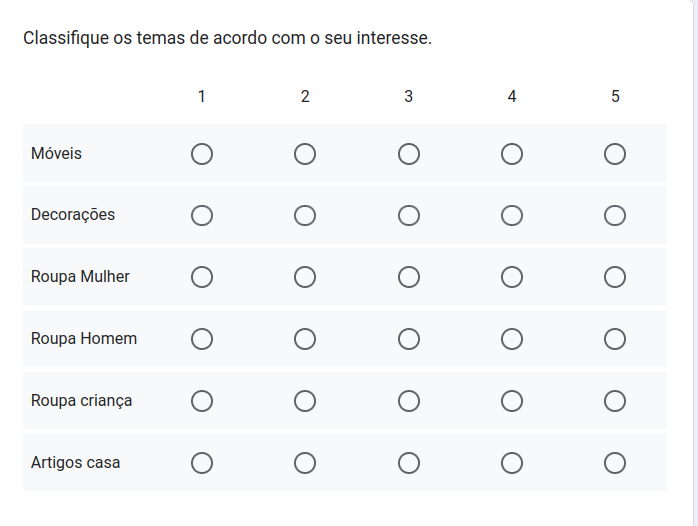
\includegraphics[width=0.75\textwidth]{form/14questao_temasinteresse.png}
    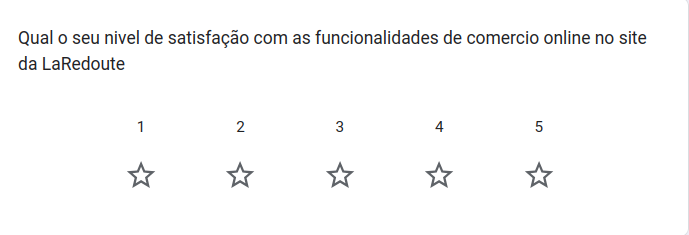
\includegraphics[width=0.75\textwidth]{form/15questao_satisfacao.png}
    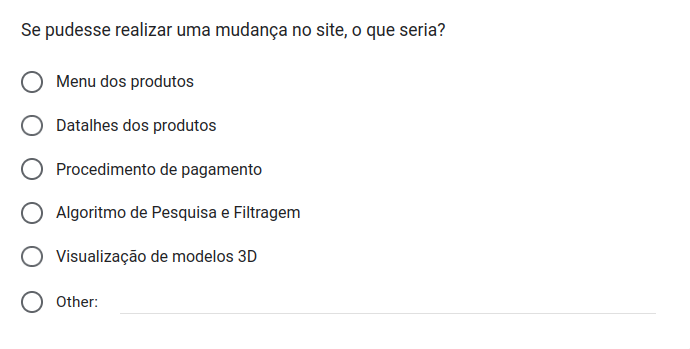
\includegraphics[width=0.75\textwidth]{form/16questao_mudancasite.png}
    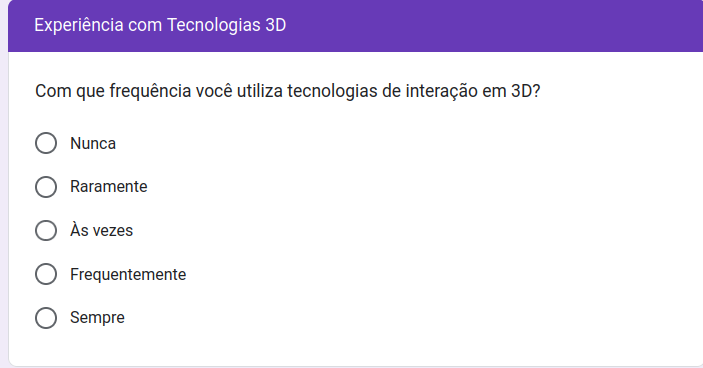
\includegraphics[width=0.75\textwidth]{form/17questao_frequencia3d.png}
    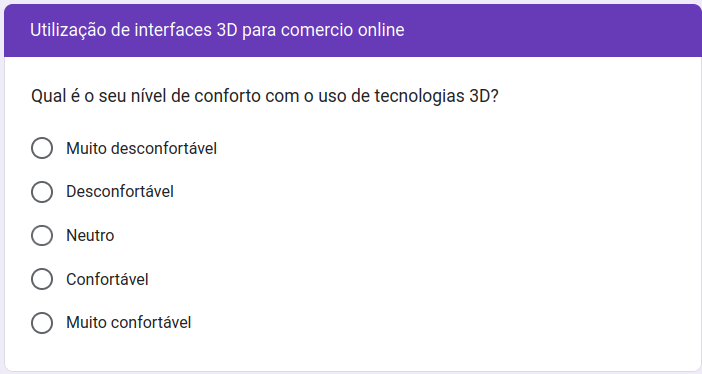
\includegraphics[width=0.75\textwidth]{form/18questao_conforto3d.png}
    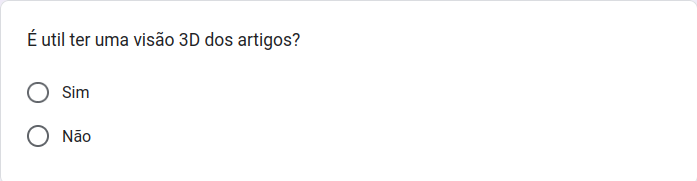
\includegraphics[width=0.75\textwidth]{form/19questao_visao3d.png}
    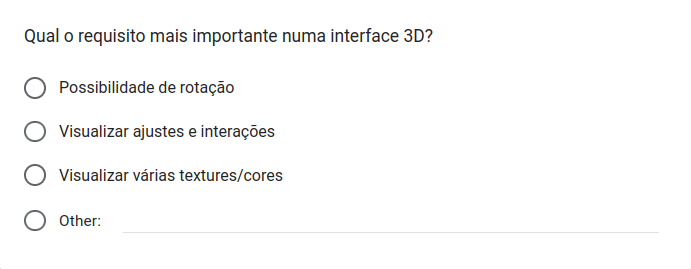
\includegraphics[width=0.75\textwidth]{form/20questao_requisito3d.png}
\end{center}

\newpage
\section{Requisitos funcionais}
Permitir que o utilizador possa:
\begin{itemize}
    \item Escolher diferentes textures
    \item Efetuar rotações ao objeto 3D
    \item Visualizar uma animação que muda o ângulo do braço do candeeiro
\end{itemize}

\subsection*{Protótipo de Alta Fidelidade}
O protótipo de alta fidelidade está disponível para consulta local nos arquivos do projeto.
Alternativamente, pode ser acedido através do seguinte link.
\begin{center}
    \textcolor{linkblue}{\href{https://www.figma.com/community/file/1456708074172973839}{Protótipo SGI}}
\end{center}

\newpage
\section{Avaliação da Usabilidade do Sistema}

Tarefas a realizar:
\begin{itemize}
    \item Aceder a págine de detalhes de um produto
          \begin{itemize}
              \item \textbf{Tempo médio gasto:} 42 segundos
              \item \textbf{Dificuldades ou Notas}: Devido a só um dos produtos levar página de detalhes, e o caroussel rodar automaticamente, os utilizadores não conseguiam aceder à página de detalhes.
          \end{itemize}
    \item Na página de detalhes do produto, interagir com o objeto 3D
          \begin{itemize}
              \item \textbf{Tempo médio gasto:} 25 segundos
              \item \textbf{Dificuldades ou Notas}: Nada a apontar
          \end{itemize}
    \item Na página de detalhes do produto, alterar a textura do objeto 3D
          \begin{itemize}
              \item \textbf{Tempo médio gasto:} 13 segundos
              \item \textbf{Dificuldades ou Notas}: Nada a apontar
          \end{itemize}
\end{itemize}

\vspace{0.5cm}

\begin{table}[h!]
    \centering
    \begin{tabular}{|m{10cm}|c|c|c|c|c|c|}
        \hline
        \textbf{Pergunta}                                                             & \textbf{1} & \textbf{2} & \textbf{3} & \textbf{4} & \textbf{5} & \textbf{Raw score} \\ \hline
        Eu acho que gostaria de usar este sistema com frequência.                     & 4          & 0          & 1          & 1          & 1          & \textbf{9}         \\ \hline
        Achei o sistema desnecessariamente complexo.                                  & 1          & 1          & 1          & 2          & 2          & \textbf{11}        \\ \hline
        Achei o sistema fácil de usar.                                                & 1          & 2          & 1          & 1          & 2          & \textbf{15}        \\ \hline
        Acho que precisaria de suporte técnico para usar este sistema.                & 2          & 0          & 0          & 3          & 2          & \textbf{11}        \\ \hline
        Achei as várias funções do sistema bem integradas.                            & 3          & 2          & 2          & 0          & 0          & \textbf{6}         \\ \hline
        Achei que havia muita inconsistência no sistema.                              & 1          & 3          & 0          & 2          & 1          & \textbf{15}        \\ \hline
        Imagino que a maioria das pessoas aprenderia a usar este sistema rapidamente. & 1          & 1          & 1          & 2          & 2          & \textbf{17}        \\ \hline
        Achei o sistema muito complicado de usar.                                     & 0          & 2          & 3          & 2          & 0          & \textbf{14}        \\ \hline
        Senti-me confiante ao usar o sistema.                                         & 2          & 3          & 0          & 1          & 1          & \textbf{10}        \\ \hline
        Precisei aprender muitas coisas antes de conseguir usar o sistema.            & 2          & 2          & 2          & 0          & 1          & \textbf{18}        \\ \hline
    \end{tabular}
\end{table}
\vspace{0.5cm}

Raw score total: 126
\vspace{0.2cm}

Número de utilizadores: 7
\vspace{0.4cm}

SUS score: \[\frac{126 * 2.5}{7} = 45\]

\newpage
\section{Análise/Discussão dos resultados}

Com base no benchmark do SUS, um score de \textbf{68} é considerado a média de usabilidade qualquer sistema. Qualquer valor abaixo deste ponto indica que o sistema possui problemas de usabilidade para o utilizador.

O score de \textbf{45} indica que o sistema se encontra na categoria de usabilidade baixa, o que sugere que existem dificuldades a interagir com o sistema.
\vspace{0.2cm}

Pode-se perceber tambem pelos scores individuais obtidos em cada pergunta que:
\begin{itemize}
    \item \textbf{Integração de funcionalidades}: A integração entre diferentes partes do sistema precisa de ser significativamente melhorada, tornando o sistema mais consistente, para garantir um fluxo mais intuitivo.
    \item \textbf{Feedback ao utilizador}: É essencial fornecer mais informações sobre o resultado de cada ação realizada, de maneira a ajudar o utilizador a entender melhor o sistema.
    \item \textbf{Adição de um FAQ}: Um conjunto de perguntas frequentes poderia ajudar os utilizadores na resolução de dúvidas e a melhorar o desempenho geral no uso do sistema.
    \item \textbf{Experiência do utilizador}: Todas estas melhorias estão diretamente ligadas a uma experiência mais agradável, que vai incentivar os utilizadores a utilizarem o sistema mais frequencia e satisfação.
\end{itemize}

Para concluir, os resultados demonstram a necessidade urgente de ajustes no sistema. Devem ser aplicadas mudanças estratégicas, baseadas nos pontos destacados, para tornar o sistema mais intuitivo, funcional e satisfatório para os utilizadores.

\newpage
\section{Principais Opções na Interface Desenvolvida}

Durante o desenvolvimento da interface, com base no site original da LaRedoute, optou-se por um design minimalista que resolve os problemas identificados na avaliação heurística do site. As principais melhorias são:

\begin{itemize}
    \item \textbf{Banner optimizado:} Reduzido em relação ao site original, para evitar que o conteúdo da página fique obscurecido.
    \item \textbf{Design mantido:} Conservação do layout dos cards para artigos individuais e do footer, por serem simples e funcionais, contendo todas as informações necessárias.
    \item \textbf{Controlo da janela 3D:} Limitação de alguns controlos na interacção com o modelo 3D, garantindo que o utilizador não saia do cenário definido.
    \item \textbf{Input numérico:} Substituição do input “select” original por um campo numérico, permitindo maior flexibilidade na alteração de quantidades.
    \item \textbf{Botões diretos:} Inclusão de botões para alterar textura/cor e categorias directamente na navbar, eliminando a necessidade de navegar por submenus.
    \item \textbf{Opção de ajustes:} Possibilidade de visualizar diferentes ajustes do artigo directamente na janela do modelo 3D.
    \item \textbf{Tabs organizadas:} Implementação de Tabs para separar descrição do produto, avaliações e especificações, reduzindo a extensão da página.
\end{itemize}

\end{document}
